% ##########################################
\begin{table*}[!ht]
  % \mnp{\textwidth}{
  \captionN{Patient Numbers, Inclusion-exclusion Criteria and Features Used In Analysis}
    \begin{subtable}{\textwidth}
  \begin{center}
    \captionN{Patient Counts In De-identified Data \& The Fraction of Datasets Excluded By Our Exclusion Criteria$^\star$}\label{tab2}
    \sffamily\small
    \begin{tabular}{L{1.5in}L{.695in}L{.695in}C{.695in}L{.695in}L{.695in}}
      &\multicolumn{2}{c@{\quad}}{Truven}    
      &&                                           
         \multicolumn{2}{c}{UCM} \\\cline{2-3}\cline{5-6}          
      Distinct Patients &\multicolumn{2}{c@{\quad}}{115,805,687}    
      &&                                           
         \multicolumn{2}{c}{69,484} \\\cline{2-3}\cline{5-6}          
      &Male& Female    && Male  &Female      \\
      \hline
      ASD Diagnosis Count$^\dag$ & 12,146 & 3,018& &307& 70 \\\hline
      Control Count$^\dag$ & 2,301,952 & 2,186,468 & & 20,249& 17,386\\\hline
      AUC at 125 weeks & 82.3\% & 82.5\% & &83.1\%& 81.37\%\\\hline
      AUC at 150 weeks & 84.79\% & 85.26\% & &82.15\%& 83.39\%\\\hline
      &&     &  &   &      \\
      \multicolumn{5}{c}{Excluded Fraction of the Data sets}      &      \\
      &&     &  &   &      \\
      \hline
      Positive Category & 0.0002 & 0.0& &0.0160& 0.0 \\\hline
      Control Category & 0.0045 &0.0045 & &0.0413&  0.0476\\\hline

      &&     &  &   &      \\
      \multicolumn{6}{c}{Average Number of Diagnostic Codes In Excluded Patients (corresponding number in included patients)}           \\
      &&     &  &   &      \\
      \hline
      Positive Category & 4.33 (35.93) & 0.0 (36.07)& &2.6 (9.75)& 0.0 (10.18) \\\hline
      Control Category & 1.57 (17.06) & 1.48 (15.96)  & & 2.32 (6.8)& 2.07 (6.79) \\\hline

    \end{tabular}
  \end{center}
    \vskip .5em
  \small
  $^\dag$ Cohort sizes are smaller than the total number of distinct patients due to the following exclusion criteria: 1) At least one code within our complete set of tracked diagnostic codes is present in the patient record, 2) Time-lag between first and last available record for a patient is at least 15 weeks.

  $^\star$ Dataset sizes are after the exclusion criteria are applied

\end{subtable}
\vskip 1em
% ###########################################################
\begin{subtable}{\textwidth}
  \captionN{Engineered Features (Total Count: 165)}\label{EXT-tab1}
  \vskip .5em

  \begin{tabular}{L{2.25in}|L{3in}|C{1in}} \hline
    \textbf{Feature Type$^\ddag$}               & \textbf{Description}   & \textbf{No. of Features}   \\\hline
    {[}Disease Category{]}$_{ \ \Delta}$               & Likelihood Defect (See Methods section) & 17   \\\hline
    {[}Disease Category{]}$_{ \ 0}$               & Likelihood of control model (See Methods section) & 17  \\\hline
    {[}Disease Category{]}$_{\textrm{ proportion}}$   & Occurrences in the encoded sequence / length of the sequence         & 17\\\hline
    {[}Disease Category{]}$_{\textrm{ streak}}$      & Maximum Length of adjacent occurrences  of {[}Disease Category{]}    & 51      \\\hline
    {[}Disease Category{]}$_\textrm{ prevalence}$   &  Maximum, mean  and variance of Occurrences in the encoded sequence / Total Number of diagnostic codes in the mapped sequence   & 51      \\\hline
    Feature Mean, Feature Variance, Feature Maximum for difference of control and case models                 & Mean, Variance, Maximum of the {[}Disease Category{]}$_{ \ \Delta}$ values   & 3     \\\hline
    Feature Mean, Feature Variance, Feature Maximum for control models               & Mean, Variance, Maximum of the {[}Disease Category{]}$_{\ 0}$ values   & 3     \\\hline
    Streak      & Maximum, mean  and variance of the length of adjacent occurrences  of {[}Disease Category{]}    & 3      \\\hline
    Intermission& Maximum, mean  and variance of the length of adjacent empty weeks     & 3    \\\hline
  \end{tabular}
  %\end{center}
  \vskip .5em
  \small
  $^\ddag$ Disease categories are described in SI-Table~\ref{SI-tab0} in Supplementary Text.
 \end{subtable}
%}
\end{table*}
% ###########################################################

% ###########################################################
\begin{figure*}[!t]

  \centering  
   
  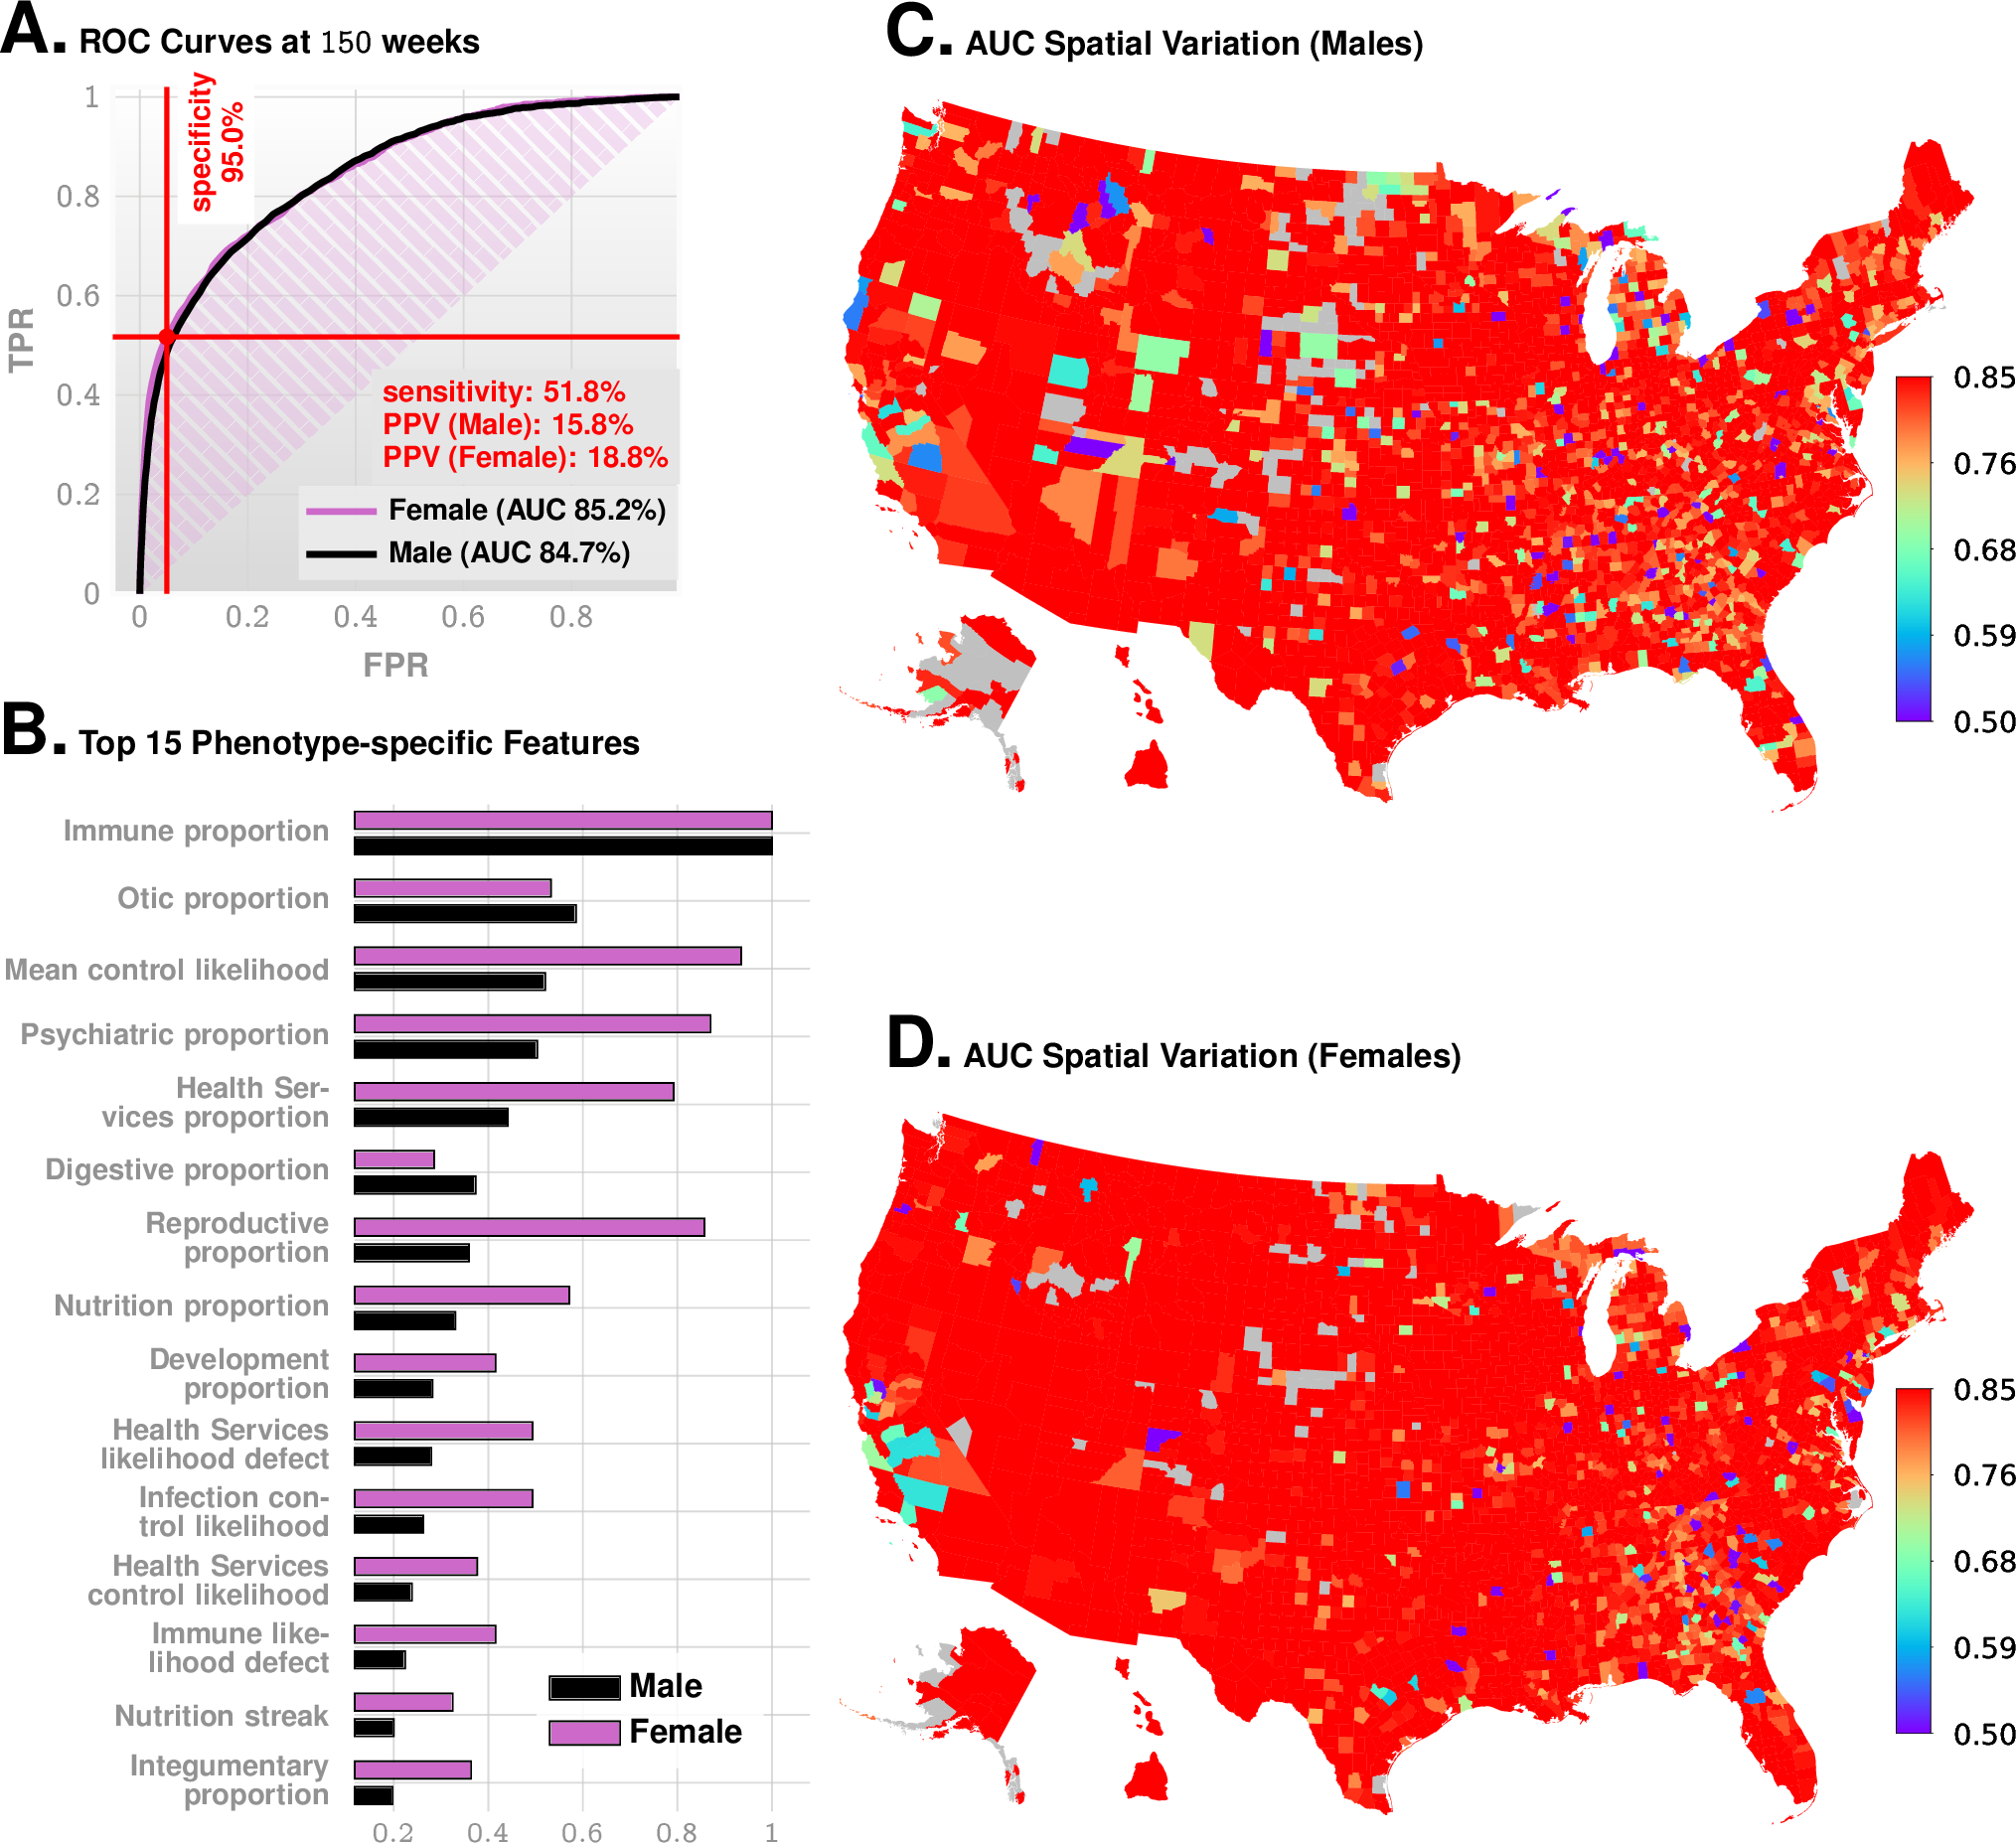
\includegraphics[width=0.85\textwidth]{Figures/External/perfA.pdf}

  \captionN{\textbf{Standalone Predictive Performance of \acor.} Panel A shows the ROC curves for males and females (Truven data shown, UCM is similar, see Fig.~\ref{fig2}a). Panel B shows the feature importance inferred by our prediction pipeline. The detailed description of the features is given in Table~\ref{EXT-tab1}. The most import feature is related to immunologic disorders, and we note that in addition to features related to individual disease categories, we also have the mean control likelihood (rank 3), which may be interpreted as the average likelihood of the diagnostic patterns corresponding to the control category as opposed to the \treatment category. Panels C and D show the spatial variation in the achieved predictive performance at 150 weeks, measured by AUC, for males and females, respectively. Gray areas lack data on either positive or negative cases. These county-specific AUC plots show that the performance of the algorithm has  relatively weak geospatial dependence, which is important in the light of the current uneven distribution of diagnostic resources. Importantly, not all counties have nonzero number of ASD patients; high performance in those counties reflects a small number of false positives with zero false negatives.
  }\label{fig1}
\end{figure*}
% ###########################################################
% ###########################################################
\begin{figure*}[!ht]
  \centering 
  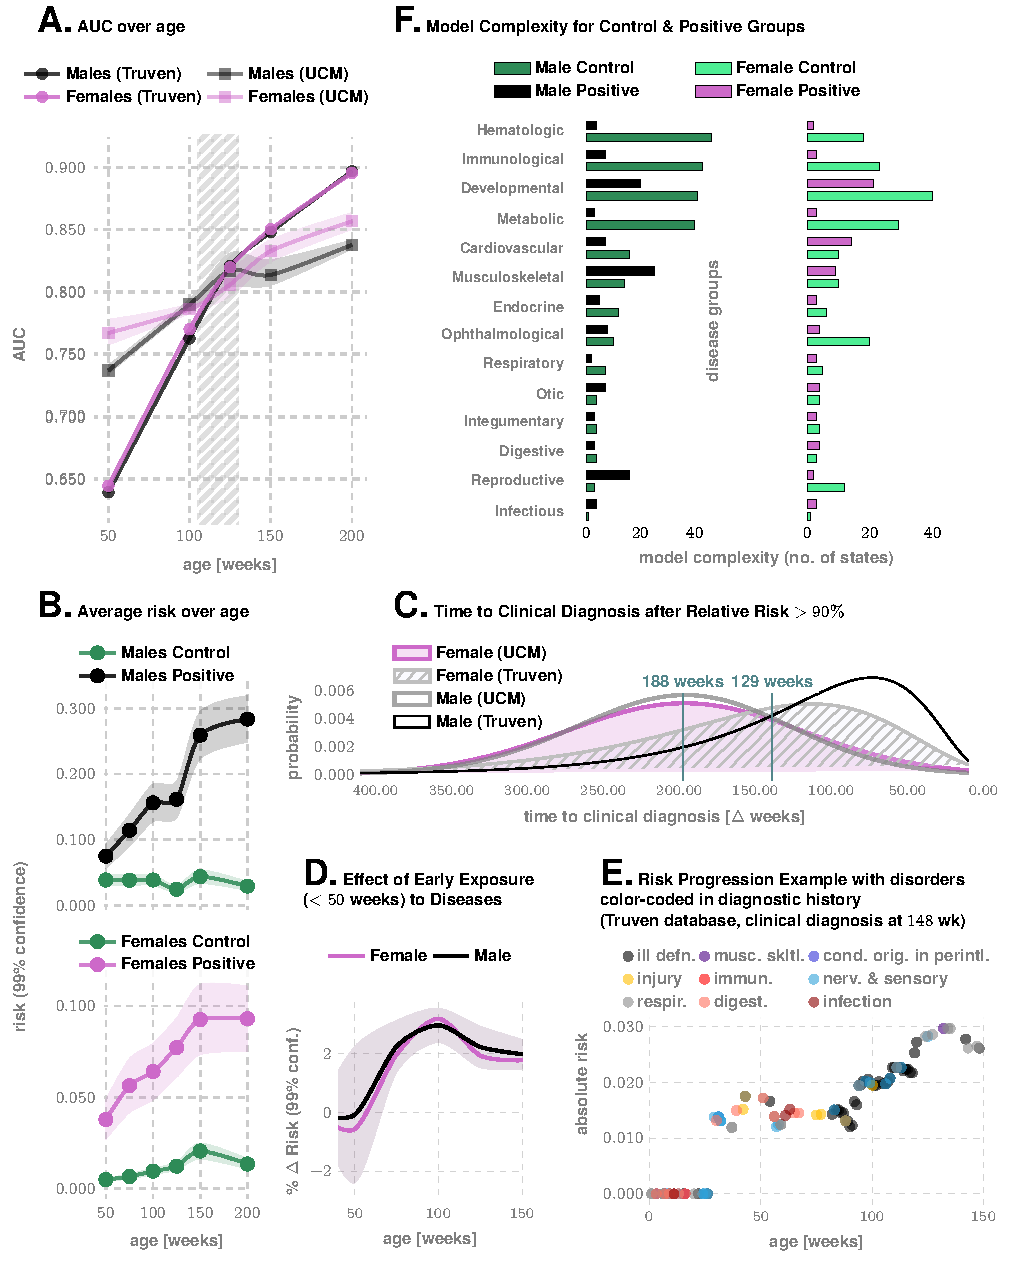
\includegraphics[width=0.85\textwidth]{Figures/External/perfB.pdf}

  \captionN{\textbf{More Details on Standalone Predictive Performance of \acor  and Variation of Inferred Risk.} Panel A illustrates AUC achieved as a function of
    patient age, for the Truven and UCM datasets. The shaded area outlines the 2 - 2.5  years of age, and  shows that we achieve $>80\%$ AUC for either sex from shortly after 2 years.   Panel B illustrates how the average risk changes with time for the control and the positive cohorts. Panel C shows the distribution of the prediction horizon: the time to a clinical diagnosis after inferred  relative risk crosses $90\%$. Panel D shows that for each new disease code for a low-risk child, ASD risk increases by approximately $2\%$ for either sex. Panel E illustrates the risk progression of a specific, ultimately autistic male child in the Truven database. Abbreviations in the legend: ill defn. (Symptoms, Signs, And Ill-Defined Conditions),   musc. skltl. (Diseases Of The Musculoskeletal System And Connective Tissue), cond. orig. in perintl. (Certain Conditions Originating In The Perinatal Period), immun. (Endocrine, Nutritional And Metabolic Diseases, And Immunity Disorders), nerv. \& sensory (Diseases Of The Nervous System And Sense Organs), respir. (Respiratory Disorders), and digest. (Digestive Disorders). Panel F illustrates  how inferred models differ between the control vs. the \treatment cohorts. On average, models get less complex, implying the exposures get more statistically independent.}\label{fig2}
\end{figure*}
% ###########################################################
\begin{figure}[!ht]
  \centering
  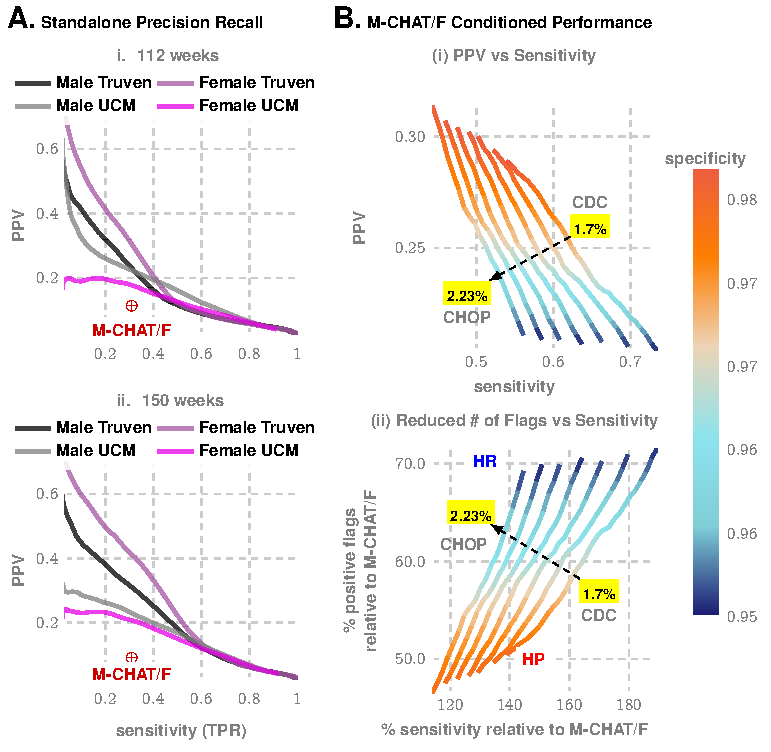
\includegraphics[width=0.75\textwidth]{Figures/External/perfCv.pdf}
 
  \captionN{\textbf{Metrics relevant to clinical practice: PPV vs Sensitivity trade-offs.} Panel A shows the precision/recall curves, $i.e.$,  the trade-off between PPV and sensitivity for \textbf{standalone operation} with \acor. Panel B shows how we can \textbf{boost \acor performance} using population stratification from the distribution of M-CHAT/F scores in the population, as reported by the CHOP study~\cite{pmid31562252}. This is possible because \acor and M-CHAT/F use independent information (co-morbidities vs questionnaire responses).  Note that the population prevalence impacts this optimization, and hence  we have  a distinct  curve for each prevalence value ($1.7\%$ is the CDC estimate, while $2.23\%$ is reported by the CHOP study).  The two extreme operating zones marked as High Precision (HP) and High Recall (HR): if we choose to operate in HR, then we do not reduce the number of positive screens by much, but maximize sensitivity, while by operating in HP, we increase sensitivity by 20-40\% (depending on the prevalence) but double the PPV achieved in current practice. In contrast, when choosing to maximize sensitivity by operating in the HR zone, we only cut down positive flags to about $70\%$ of what we get with M-CHAT/F, but boost sensitivity by $50-90\%$ (Reaching sensitivities over $70\%$). Note in all these zones, we maintain specificity above $95\%$, which is the current state of art, implying that by doubling the PPV, we can halve the number of positive screens currently reported, thus potentially sharply reducing the queues and wait-times. }\label{figprc} 
\end{figure}
% ####################################
\def\RCOL{\rowcolor{teal!40}}
\def\PCOL{Tomato!40}
%#################################### 
\begin{table*}[!ht]
  \captionN{Standalone \acor Performance and Boosted Performance Conditioned on M-CHAT/F}
\begin{subtable}{\textwidth}
\centering 
\captionN{Standalone PPV Achieved at 100, 112 and 150 Weeks For Each Dataset and Gender {\bf (M-CHAT/F:  sensitivity=$38.8\%$, specificity=$95\%$, PPV=$14.6\%$ between 16 and  26 months ($\approx$112 weeks))}}\label{EXT-tabssp}

  \vskip .5em

\begin{tabular}{L{.75in}|L{.75in}|L{.75in}|L{.5in}|L{.5in}|L{.75in}}
\hline

weeks&specificity&sensitivity&PPV&gender&dataset\\\hline
100&0.92&0.39&0.14&F&UCM\\\hline
100&0.95&0.39&0.19&M&UCM\\\hline
100&0.93&0.39&0.13&F&Truven\\\hline
100&0.91&0.39&0.10&M&Truven\\\hline
\RCOL 112&0.93&0.39&0.16&F&UCM\\\hline
\RCOL 112&0.95&0.39&0.20&M&UCM\\\hline
\RCOL 112&0.96&0.39&0.22&F&Truven\\\hline
\RCOL 112&0.95&0.39&0.17&M&Truven\\\hline
150&0.94&0.39&0.19&F&UCM\\\hline
150&0.98&0.39&0.34&F&Truven\\\hline
150&0.97&0.39&0.26&M&Truven\\\hline
150&0.97&0.39&0.26&M&UCM\\\hline

  
\end{tabular}\end{subtable}
\vskip 1em
\begin{subtable}{\textwidth}
\centering
\captionN{Personalized Operation Conditioned on M-CHAT/F Scores at  26 months}\label{EXT-tabboost}
  \vskip .5em

\begin{tabular} {L{.33in}|L{.33in}|L{.33in}|L{.33in}||L{.35in}|L{.35in}|L{.375in}||L{.375in}|L{.35in}|L{.35in}||L{.6in}}
\hline
\multicolumn{4}{c||}{\cellcolor{lightgray!60}M-CHAT/F Outcome}  & \multicolumn{3}{c||}{\mnp{1.2in}{\vskip .2em global performance (Truven)\vskip .2em  } }&\multicolumn{3}{c||}{\mnp{1.2in}{\vskip .2em global performance\\(UCM)\vskip .2em }} &  \multirow{3}{*}{prevalence$^\star$}\\\cline{0-9}
 0-2  NEG & 3-7  NEG & 3-7  POS & $\geq  8$  POS & \multirow{2}{*}{\mnp{.1in}{speci-ficity}} & \multirow{2}{*}{\mnp{.1in}{sensi-tivity}} &\multirow{2}{*}{PPV}& \multirow{2}{*}{\mnp{.1in}{speci-ficity}} & \multirow{2}{*}{\mnp{.1in}{sensi-tivity}} & \multirow{2}{*}{PPV} & \\\cline{0-3}
\multicolumn{4}{c}{\cellcolor{lightgray} specificity choices}  & & & &&&&\\\hline 

0.2&0.54&0.83&0.98&0.95&0.585&0.209&0.95&0.505&0.186&0.022\\\hline 
0.21&0.53&0.83&0.98&0.95&0.586&0.208&0.95&0.506&0.184&0.022\\\hline 
0.42&0.87&0.98&0.99&\cellcolor{\PCOL}0.98&\cellcolor{\PCOL}0.433\cellcolor{\PCOL}&\cellcolor{\PCOL}0.331&0.98&0.347&0.284&0.022\\\hline 
0.48&0.87&0.97&0.99&\cellcolor{\PCOL}0.98&\cellcolor{\PCOL}0.432&\cellcolor{\PCOL}0.331&0.98&0.355&0.289&0.022\\\hline 
0.38&0.54&0.94&0.98&\cellcolor{\PCOL}0.95&\cellcolor{\PCOL}0.736\cellcolor{\PCOL}&\cellcolor{\PCOL}0.203&0.95&0.628&0.178&0.017\\\hline 
0.3&0.55&0.94&0.98&\cellcolor{\PCOL}0.95&\cellcolor{\PCOL}0.737&\cellcolor{\PCOL}0.203&0.95&0.633&0.179&0.017\\\hline 
0.58&0.96&0.98&0.99&0.98&0.492&0.302&0.98&0.373&0.247&0.017\\\hline 
0.59&0.96&0.98&0.99&0.98&0.491&0.303&0.98&0.372&0.248&0.017\\\hline 
0.46&0.92&0.97&0.99&0.977&0.534&0.291&0.977&0.448&0.256&0.017\\\hline 
0.48&0.92&0.97&0.99&0.978&0.533&0.292&0.978&0.448&0.257&0.017\\\hline 

  
\end{tabular}
\vskip 1em

\flushleft
$^\star$Prevalence reported by CDC is $1.7\%$, while the CHOP study reports a value of $2.23\%$. The results of our optimization depend on the prevalence estimate.
\end{subtable}
\end{table*}  
%####################################
%###########################################################
\begin{figure*}[!t]
\centering
  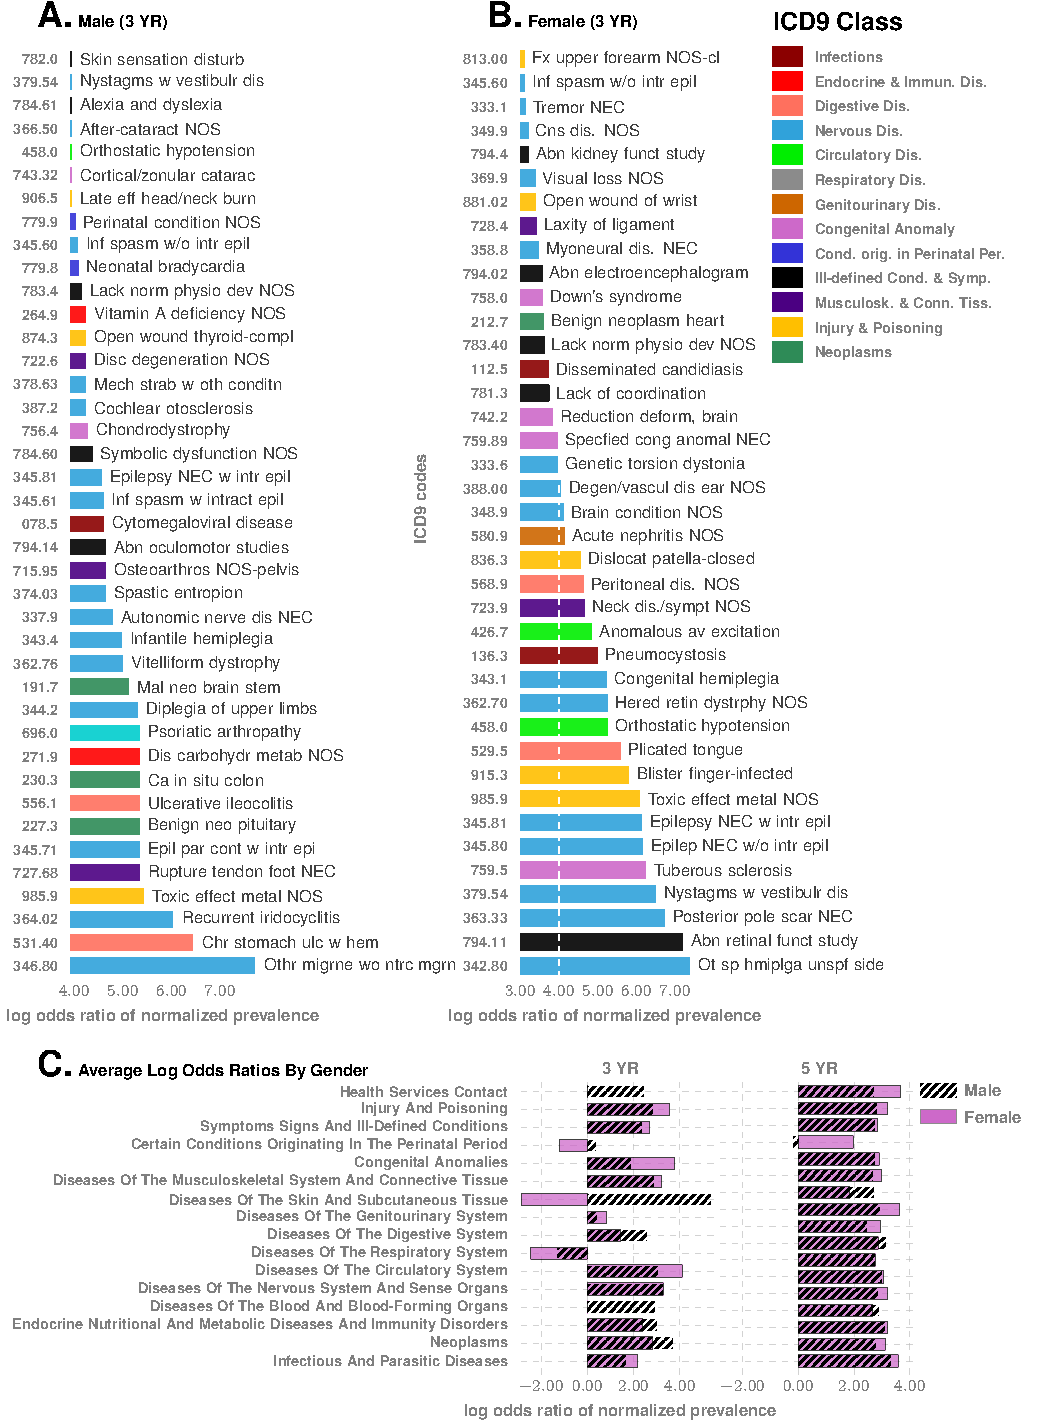
\includegraphics[width=0.9\textwidth]{Figures/External/comorbidA}
 
  \captionN{\textbf{Co-morbidity Patterns} Panel A and B. Difference in occurrence frequencies of diagnostic codes between true positive (TP) and true negative (TN) predictions. The dotted line on panel B shows the  abscissa lower cut-off in Panel A, illustrating the lower prevalence of codes in females. Panel C illustrates log-odds ratios for ICD9 disease categories at different ages. Importantly, the negative associations disappear when we consider older children, consistent with the lack of such reports in the literature which lack studies on very young cohorts. }\label{EXT-fig3}
\end{figure*}
